%!TEX root = ../main.tex
% chktex-file 13

\subsection{Approaches}\label{sec:approaches}

The approach taken to port a code to SYCL or OneAPI\cite{intel_corp_oneapi_nodate} depends on various factors including the programming language of the original codebase and whether or not there are already directives used. Intel's recommendations (See fig:\ref{fig:intel-workflow}) include a flowchart illustrating this.

\begin{figure}[htb]
	\caption{Intel's Recommended Workflow}
	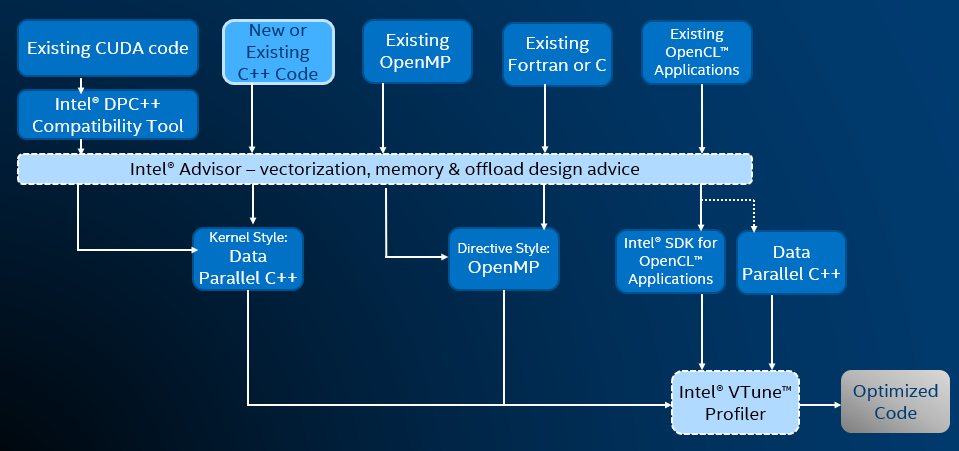
\includegraphics[width=\textwidth]{intel-oneapi-workflow.png}
	\label{fig:intel-workflow} % chktex 24
\end{figure}

\subsection{Hardware Platforms}

DiRAC has several platforms available that provide GPUs. DiRAC has access to a portion of CSD3 at Cambridge whose Wilkes-3 partition has 80 nodes of Dell XE8545 each containing four Nvidia A100 80 GiB GPUs. As part of the ExCALIBUR project the COSMA system at Durham hosts a testbed including a server with six AMD MI50 GPUs.

The porting project also has access to the Intel DevCloud which is operated on Intel's behalf by Colfax. There are a variety of Intel GPUs available from the Iris XE integrated graphics to the DG1 (discrete graphics) Arctic Sound GPU available to some customers on an NDA (non disclosure agreement) basis.

\begin{table}[htbp]
	\centering
	\begin{tabular}{lllll}
		Cluster  & Vendor & GPU Model        & GPUs / node & GPU nodes \\
		\hline  % chktex 44
		CSD3     & Nvidia & A100             & 4           & 80        \\
		COSMA8   & AMD    & MI50             & 6           & 1         \\
		DevCloud & Intel  & Iris XE          & 1           & 13        \\
		DevCloud & Intel  & DG1 Arctic Sound & 1,2 or 4    & 2
	\end{tabular}
	\caption{Hardware platforms available to the project}
	\label{tab:GPUs} % chktex 24
\end{table}

\subsection{Software Stack}

The project has access to Intel's OneAPI \texttt{dpcpp} version 2022.0.0 on both CSD3 and the DevCloud. These compilers can target Intel GPUs and any x86\_64 CPU. On CSD3 we have a locally built version of the open source Intel Project for LLVM technology which can target Nvidia A100 GPUs and x86\_64 CPUs.

We have hipSYCL version 0.9.1 on CSD3 that can target A100 GPUs and it would be possible to build hipSYCL on COSMA8 to target AMD GPUs.

The version of CUDA installed on CSD3 is 11.4 and on COSMA the version of ROCm is 5.0.1 and the version of HIP is 5.0.13601-bb16828d.

\begin{figure}[htbp]
	\caption{The SYCL~(\cite{kronos_group_sycl_nodate}) Landscape}
	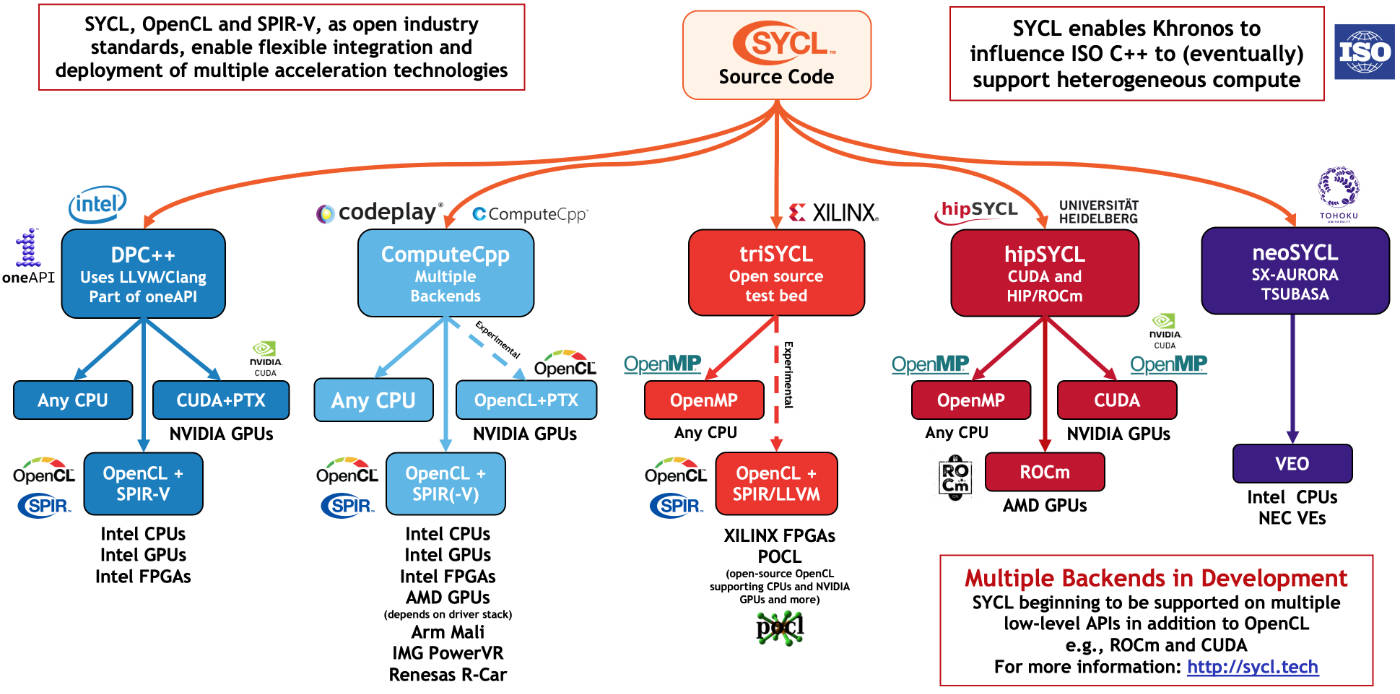
\includegraphics[width=\textwidth]{2020-05-sycl-landing-page-02_3.jpeg} % chktex 8
	\label{fig:sycl-landscape} % chktex 24
\end{figure}
